% Author: Taejin Hwang, Maxwell Chen
% Email: taejin@berkeley.edu, maxhchen@berkeley.edu

\qns{Principal Component Analysis}

Given a dataset with very high dimensions, we want to see if it is possible to represent this data using much fewer dimensions. 
Principal Component Analysis or PCA is a process that takes a data matrix containing values of different variables, and converts them into an orthogonal set of \textbf{principal components}, each weighted by importance from smallest to largest.

The principal components, and PCA can be interpreted as solving the following problems:
\begin{itemize}
  \item Given a dataset of rank $n >> k,$ how can I approximate this dataset using a matrix of only rank $k.$
  \item If I we were to project the data onto the unit circle, where $\norm{\vec{x}} = 1,$ which $\vec{x}$ would maximize $\norm{A \vec{x}}?$
\end{itemize}

We showed in the previous question that $A_{k} = \sum\limits_{i = 1}^{k} \sigma_{i} \vec{u}_{i} \vec{v}_{i}^{T}$ solves the first problem, and the eigenvector of largest eigenvalue of $A^{T}A,$ $\vec{v}_{1}$ solves the second problem. Therefore, we will utilize the SVD in order to perform PCA for a matrix $A$ through the following process:
\begin{itemize}
  \item Normalize $A$ by calculating the mean $\mu_{i}$ of each row and subtracting it from every value in the row. The resulting matrix is denoted as $\tilde{A}$, centering our data at the mean (graphically setting (0,0) to be the mean).
  \item Find the SVD of $\tilde{A}$ such that $\tilde{A} = U \Sigma V^T$. It may be helpful to refer to last week's worksheet for computing the SVD.
  \item The principal components will be the vectors in the $V$ matrix of the SVD of $\tilde{A}.$ 
  Usually only the first few vectors are taken from this $V$ matrix, since we want to represent our data with as few dimensions as possible.
\end{itemize}

In this question, we will look at how to compute a Principal Component Analysis, but also build some intuition on how to visualize the dimensionality reduction.

\meta {
  Note that it is convention to aggregate data by rows in PCA. We will discuss column aggregation in part (d).
}

\begin{enumerate}
	\qitem Find the Principal Components for the following matrix representing 2 variables each with 3 values: 
  $$A = \begin{bmatrix}
    5 & -6 \\ 
    7 & 0 \\
    11 & -4 \\
    5 & -6
  \end{bmatrix}$$

  Visually the data will look like the following:
  \begin{center}
    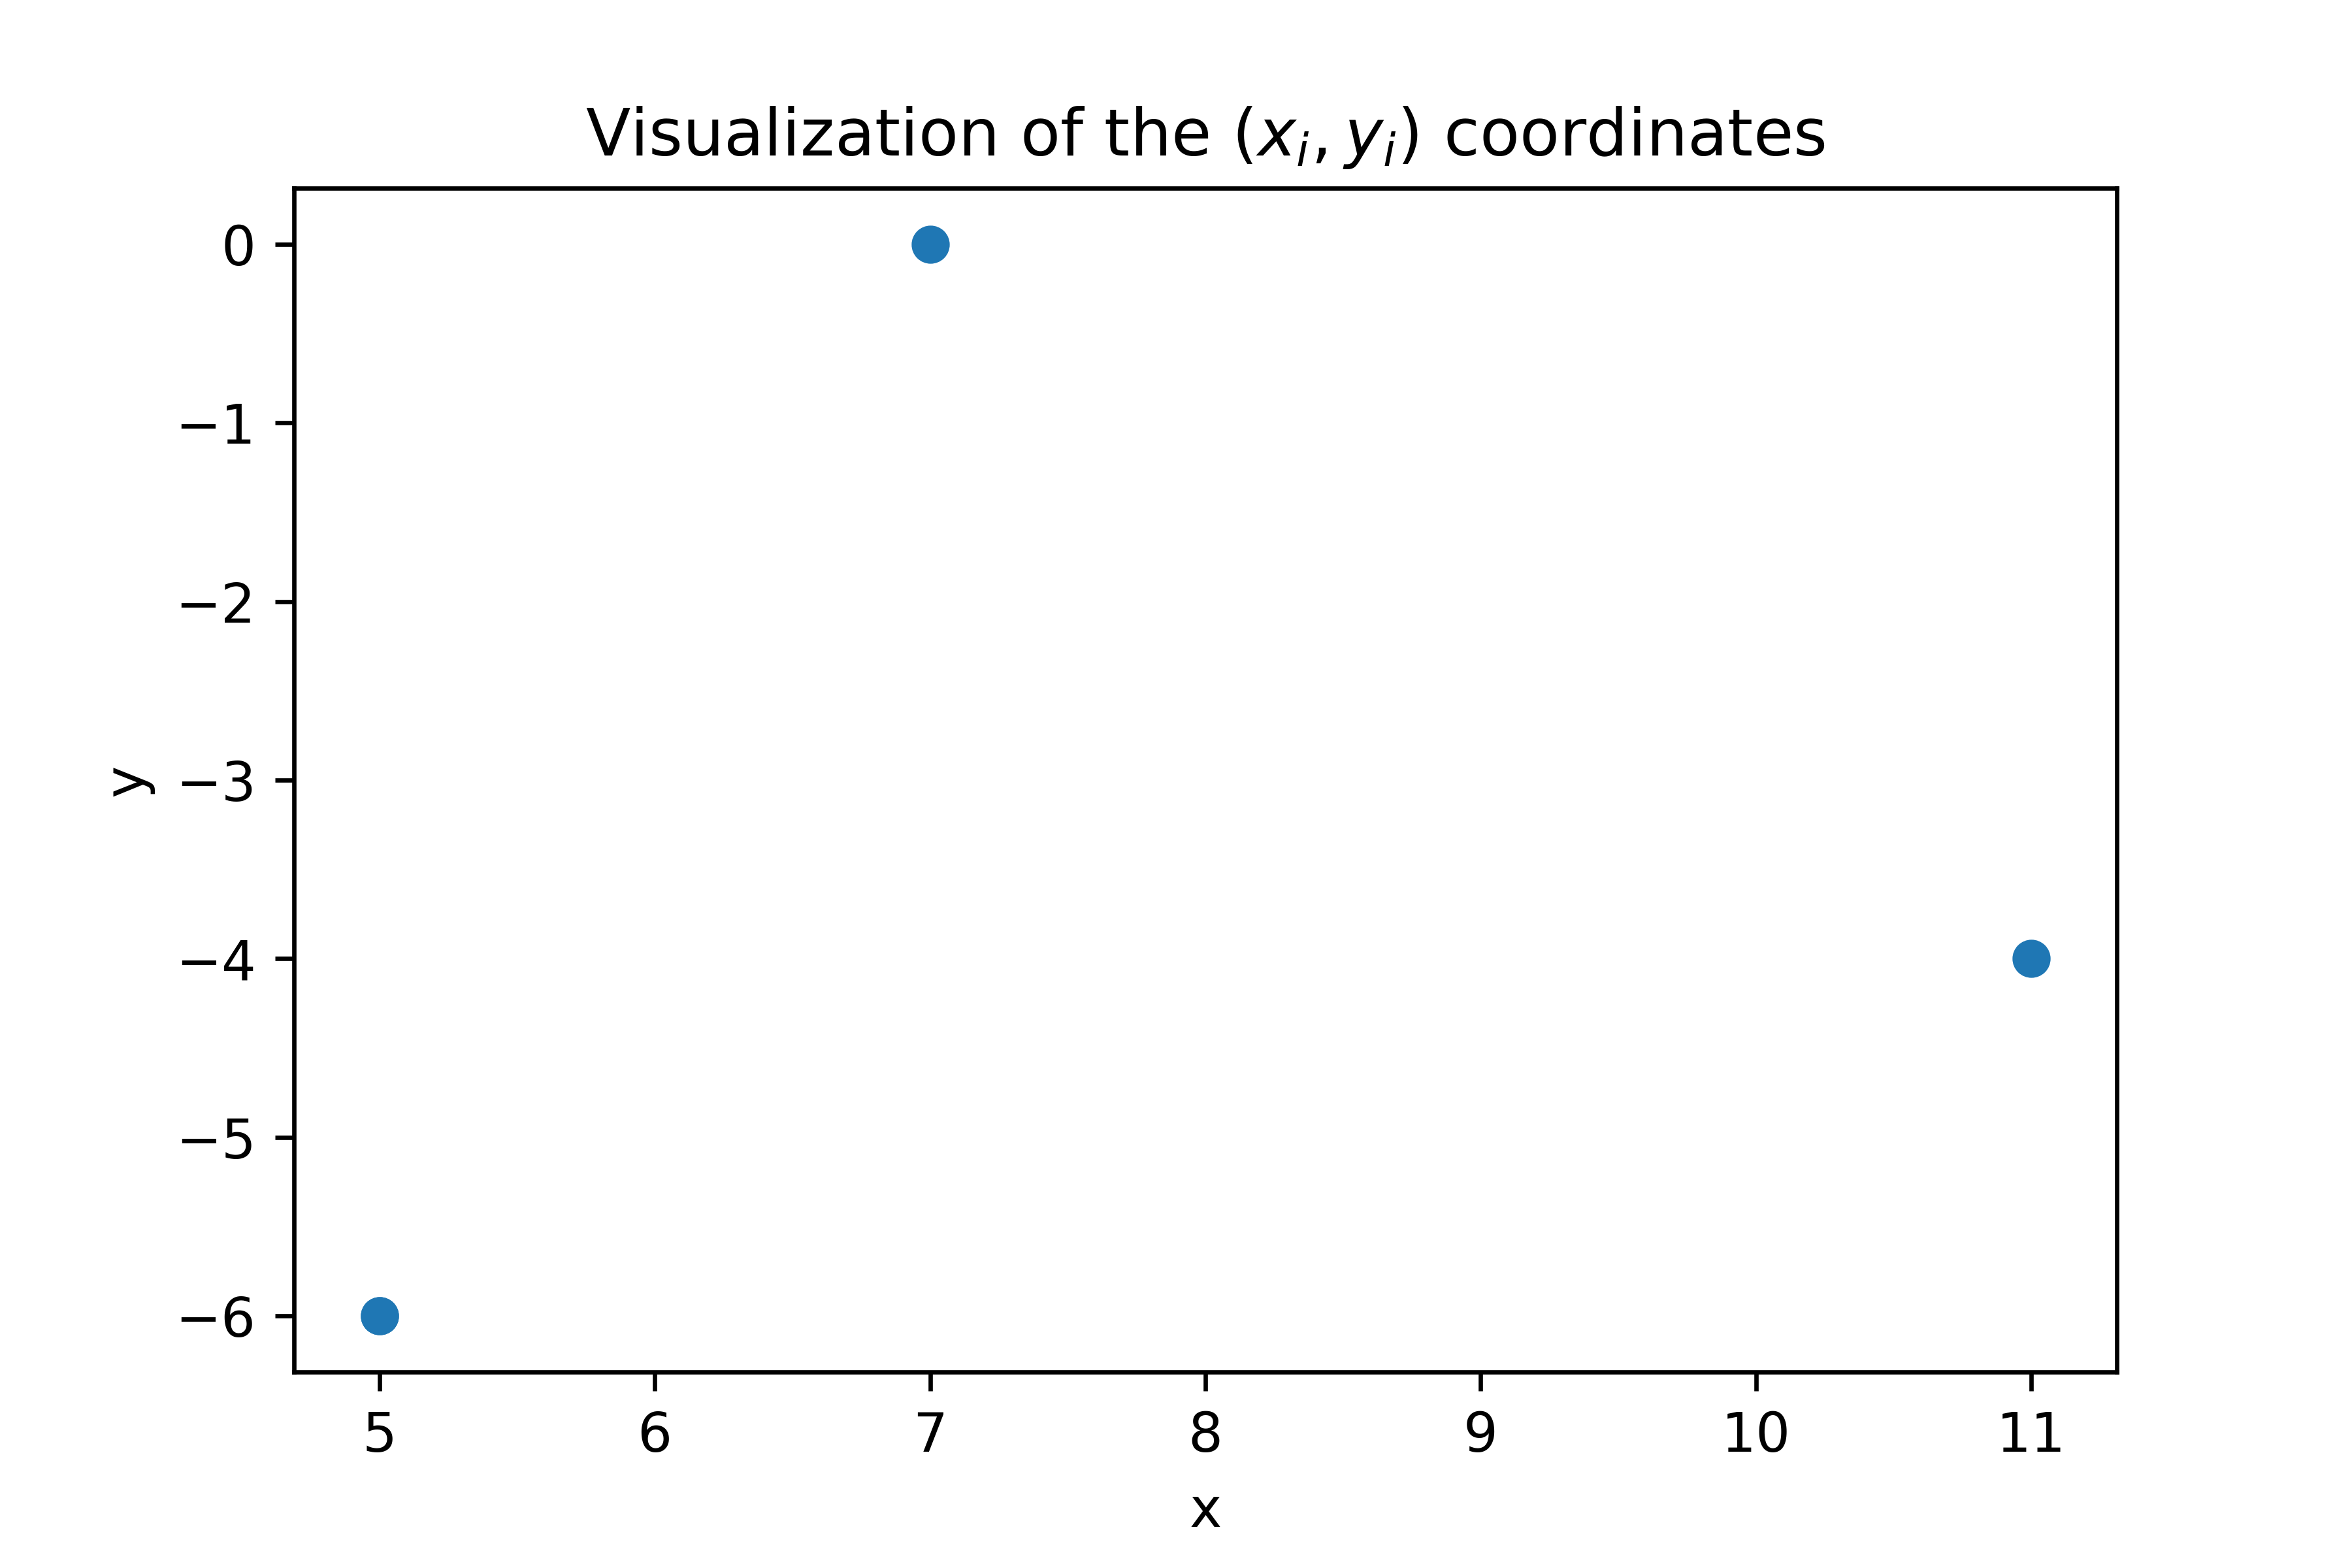
\includegraphics[width=4in]{\bank/svd-pca/figures/mech_pca.png}
  \end{center}

  \meta {
    After finishing this mechanical question, draw out the principal components so students can see which direction they are pointing in.
  }

	\sol {
    The mean of the first column is $\mu_{1} = \frac{5 + 7 + 11 + 5}{4} = 7,$ and the mean of the second column is $\mu_{2} = \frac{-6 + 0 - 4 - 6}{4} = -4.$
    Therefore, our demeaned matrix will be:
    $$\widetilde{A} = \begin{bmatrix}
    -2 & -2 \\
    0 & 4 \\
    4 & 0 \\
    -2 & -2 
    \end{bmatrix}$$
    We will now find the SVD of this matrix. Remember that this can be done by looking at the eigenvectors and eigenvalues of the matrix $A^{T} A.$
    $$A^{T} A = \begin{bmatrix}
    24 & 8 \\
    8 & 24
    \end{bmatrix}$$
    The eigenvalues of this matrix will be: $(\lambda - 24)^{2} - 64 = \lambda^{2} - 48 \lambda + 576 - 64 = (\lambda - 16)(\lambda - 32).$ Therefore the eigenvalues will be $\lambda_{1} = 32, \lambda_{2} = 16.$ 
    Now we compute the eigenvectors of $A^{T} A:$ 
    $$A - 32I = 
    \begin{bmatrix}
    -8 & 8 \\
    8 & -8 
    \end{bmatrix}$$
    Computing the null-space we see that $\vec{v}_{1} = \begin{bmatrix} 1 / \sqrt{2} \\ 1 / \sqrt{2} \end{bmatrix}.$
    $$A - 16I = 
    \begin{bmatrix}
    8 & 8 \\
    8 & 8
    \end{bmatrix}
    $$
    Computing the null-space we see that $\vec{v}_{2} = \begin{bmatrix} 1 / \sqrt{2} \\ -1 / \sqrt{2} \end{bmatrix}.$

    We could compute the $U$ vectors to finish up the SVD, but we only need the vectors in the $V$ matrix to perform our Principal Component Analysis. Therefore, our principal components will be $\vec{v}_{1}$ and $\vec{v}_{2}.$

    We conclude by showing a plot of the first principal component.
    \begin{center}
      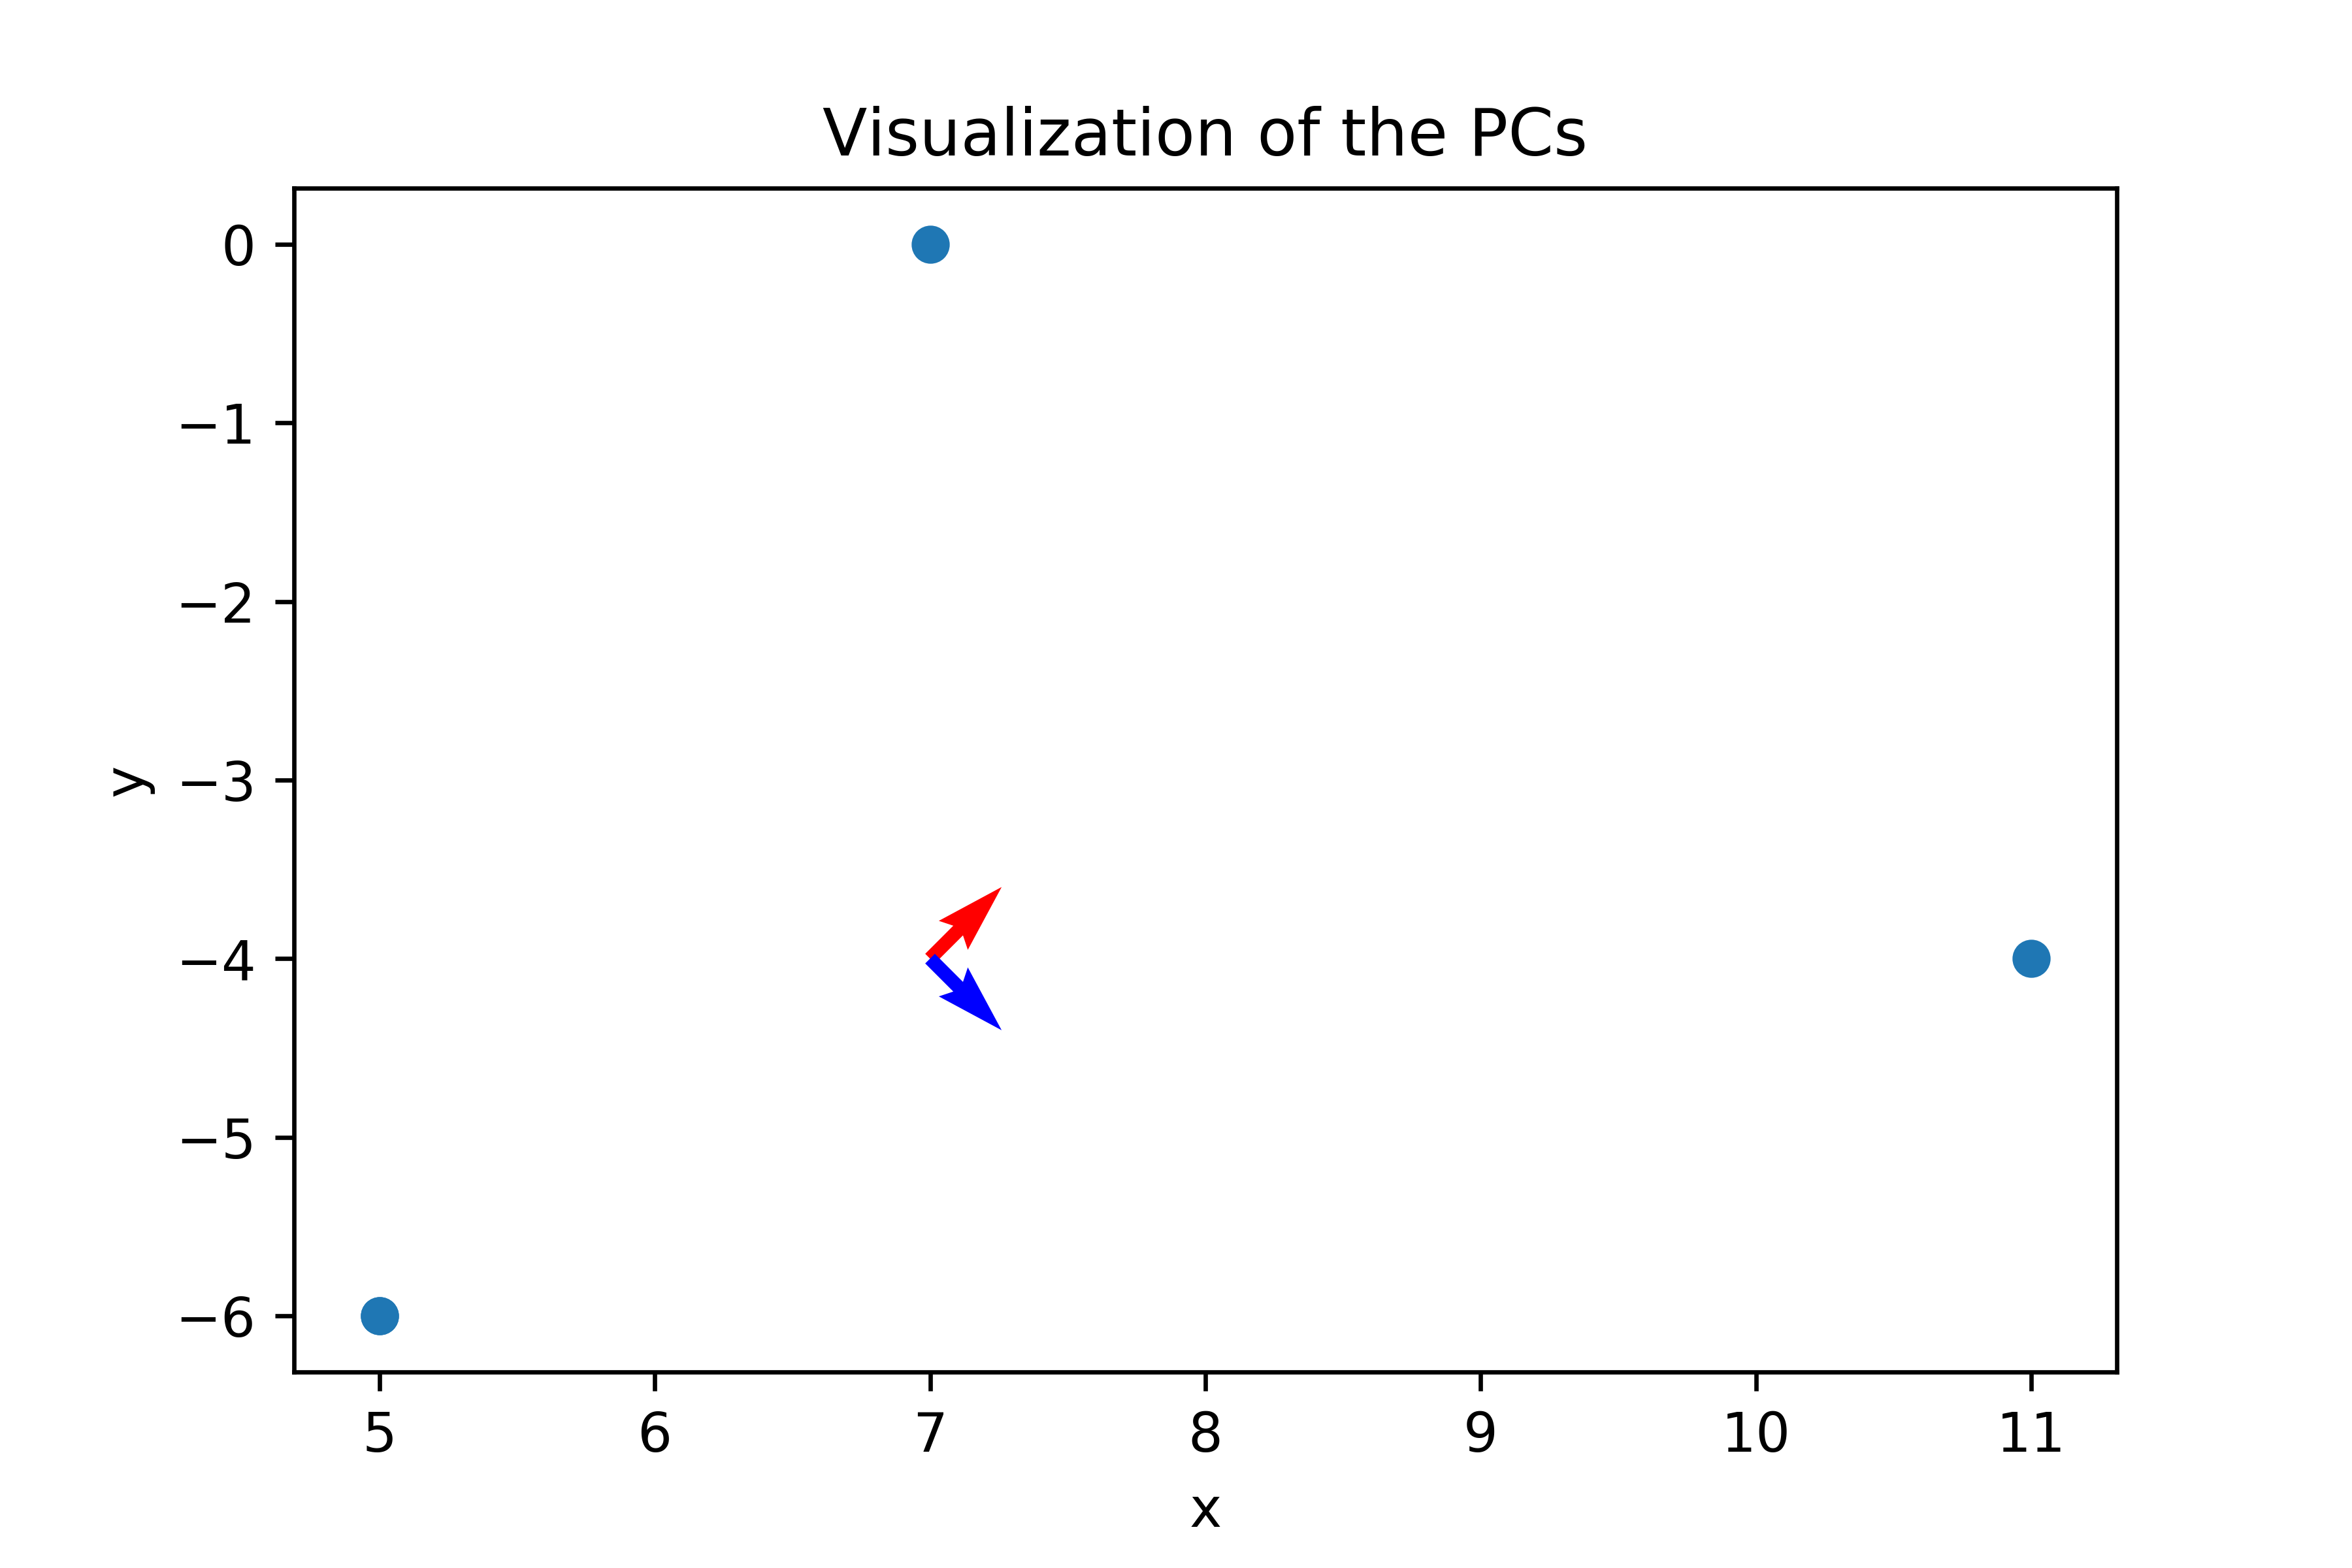
\includegraphics[width=4in]{\bank/svd-pca/figures/mech_pca_pc1.png}
    \end{center}
	}

	\qitem Given the following 2D dataset below, draw the direction of the first principal component, and its span.

  \begin{center}
    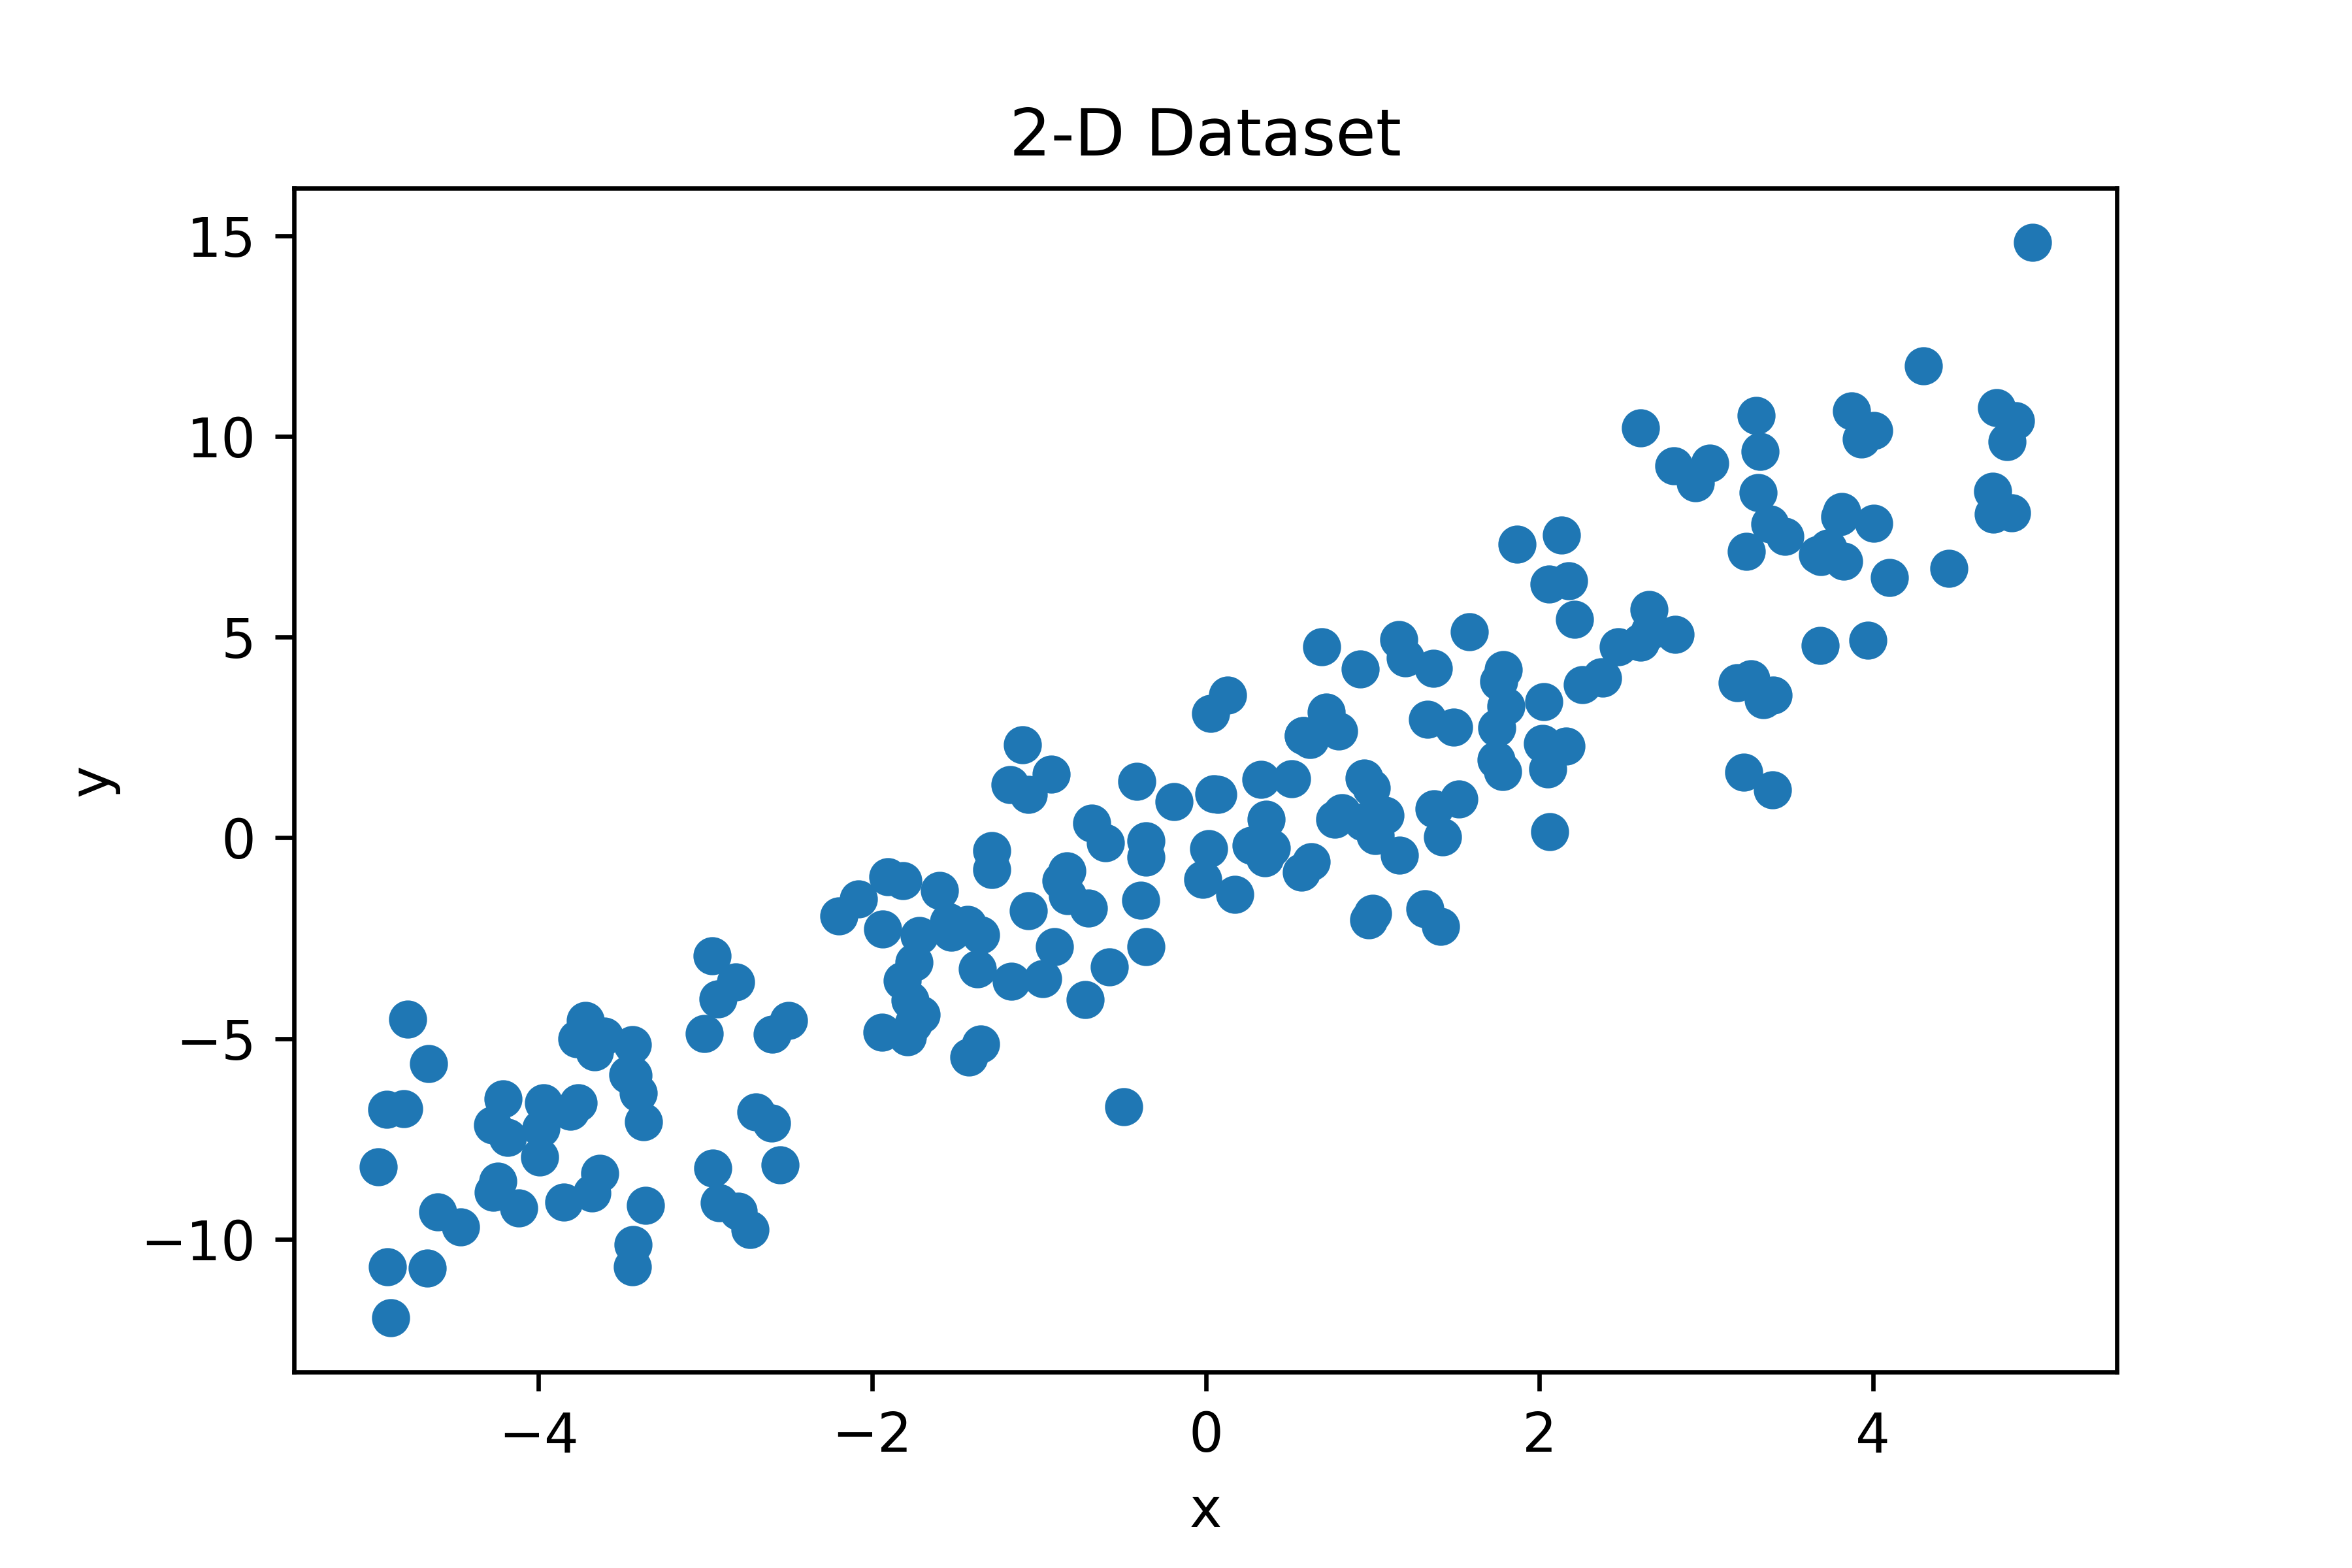
\includegraphics[width=4in]{\bank/svd-pca/figures/2d_data.png}
  \end{center}

	\sol {
    Looking at the data, we should try to draw the first principal component centered at the mean, and in the direction of maximal spread. 
    \begin{center}
      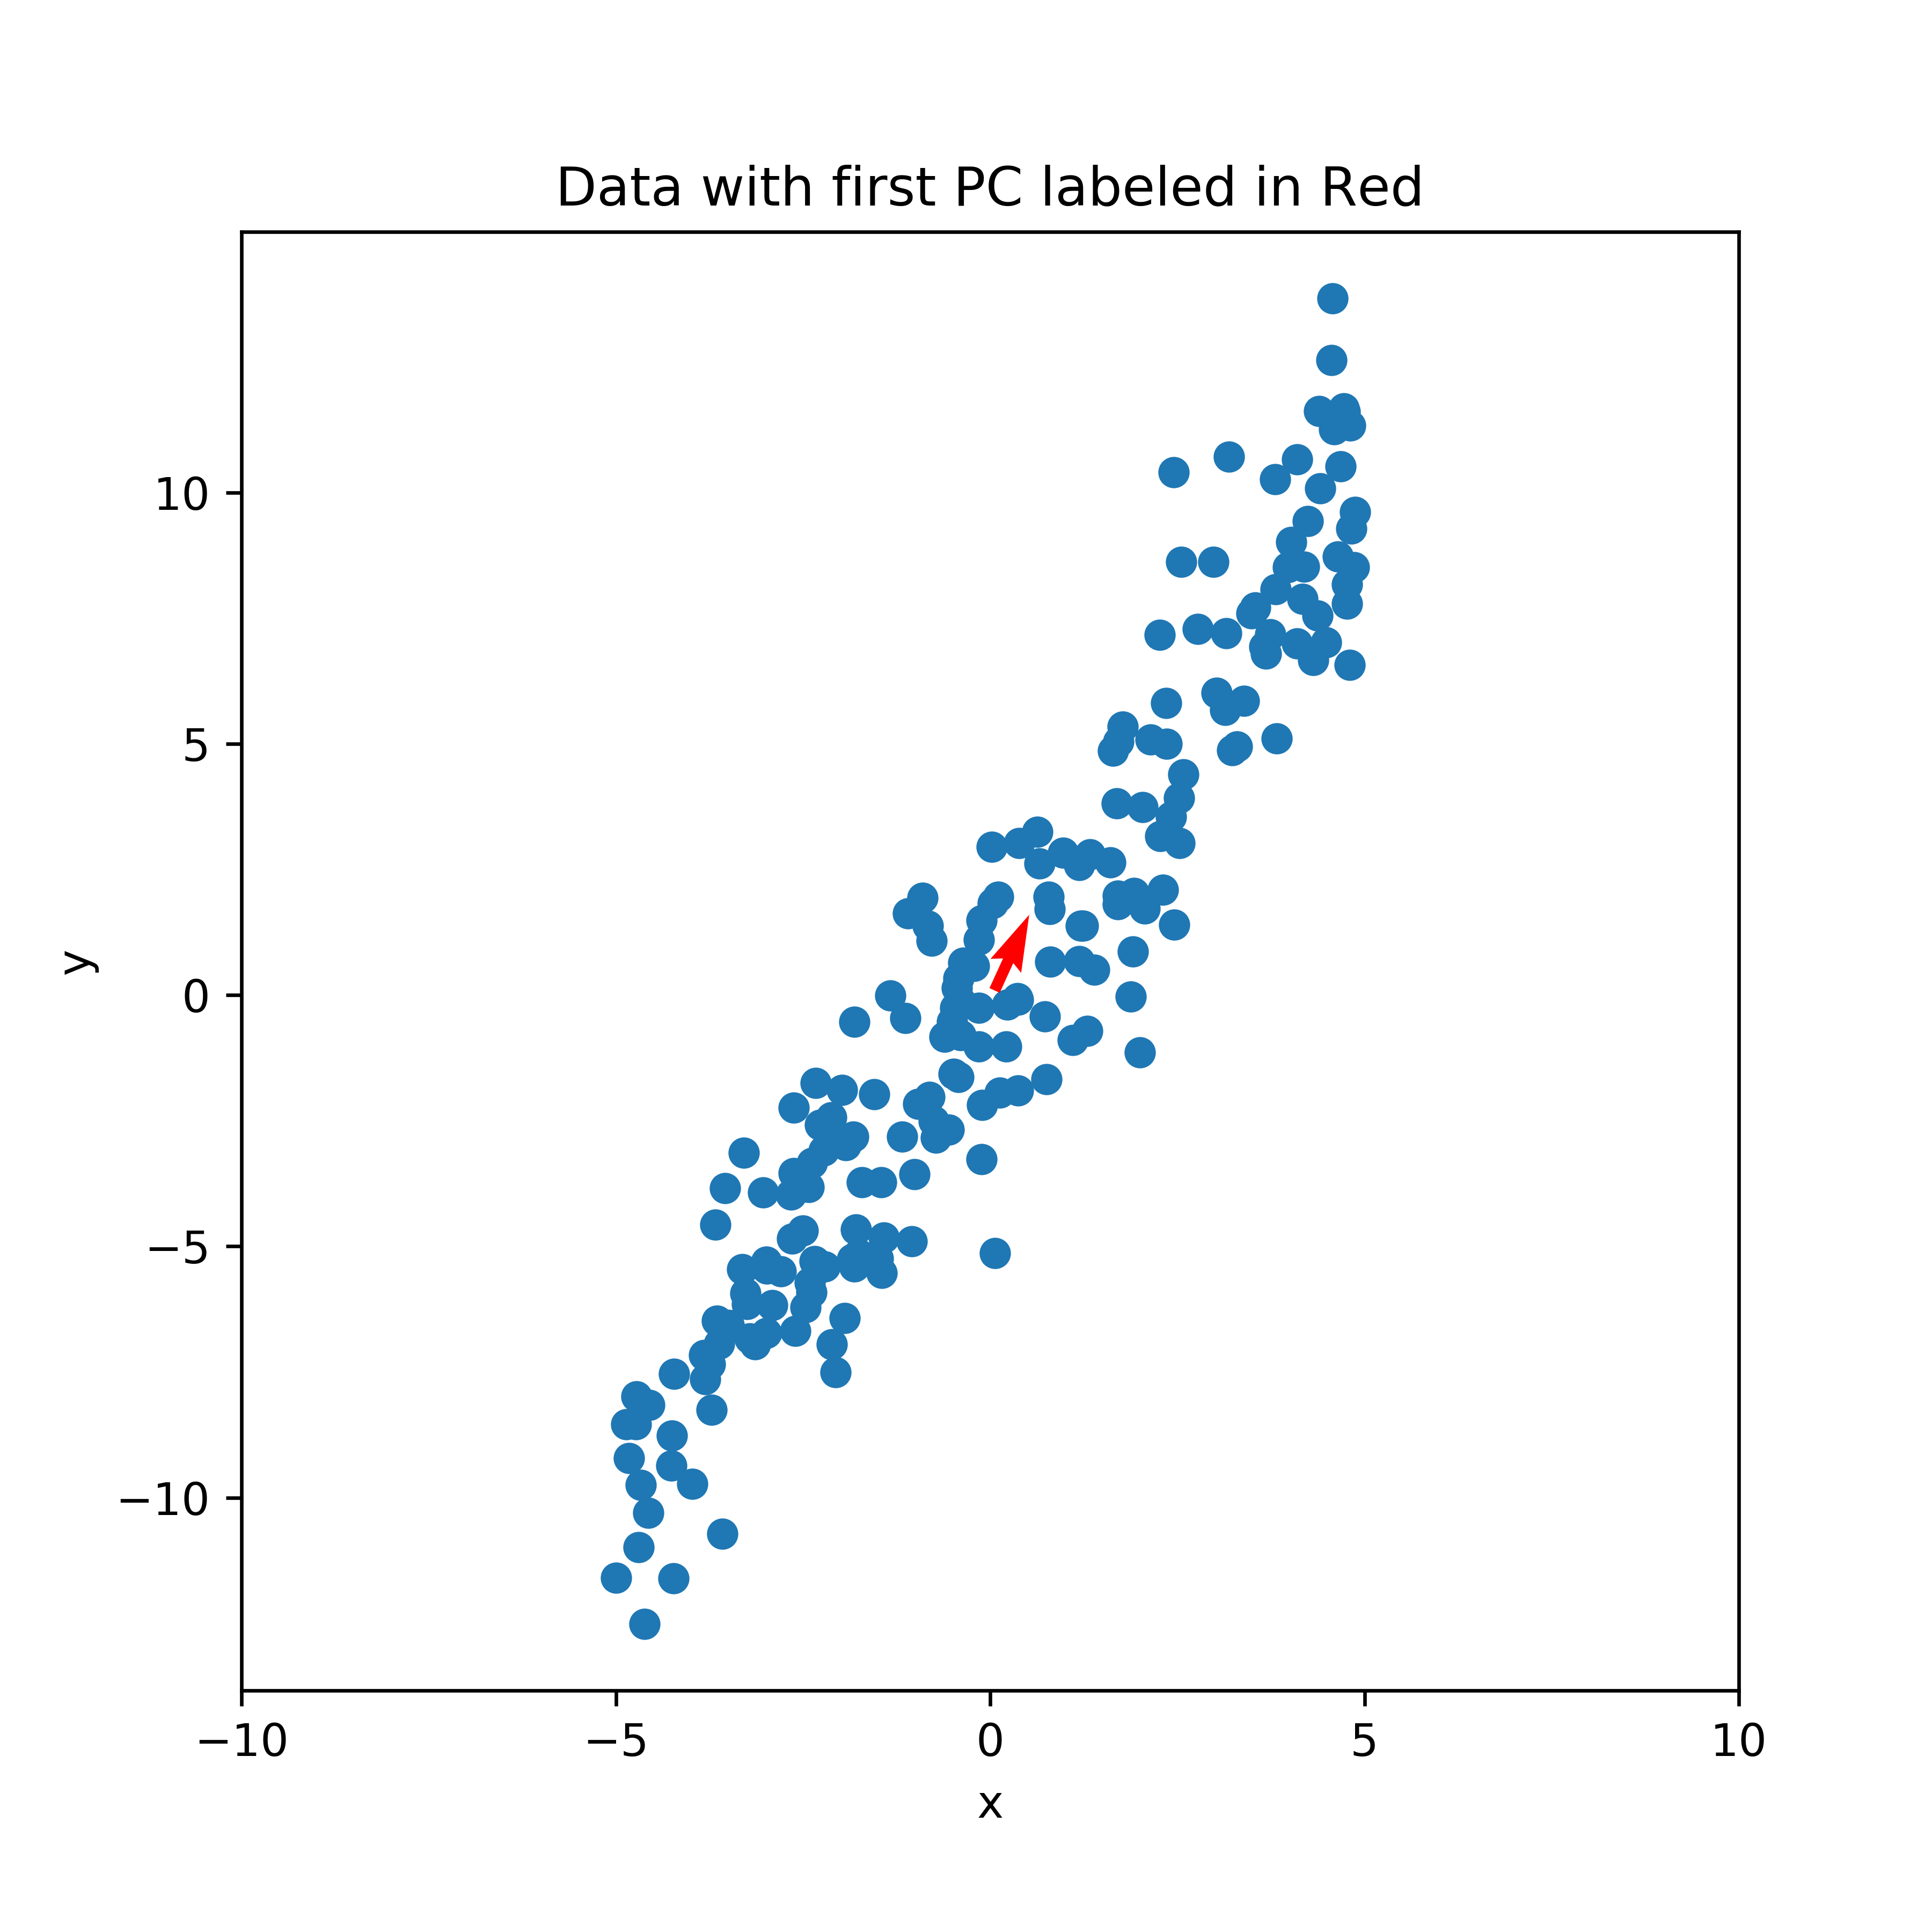
\includegraphics[width=4in]{\bank/svd-pca/figures/2d_data_pc1.png}
    \end{center}

    It's span will also look like the following:
    \begin{center}
      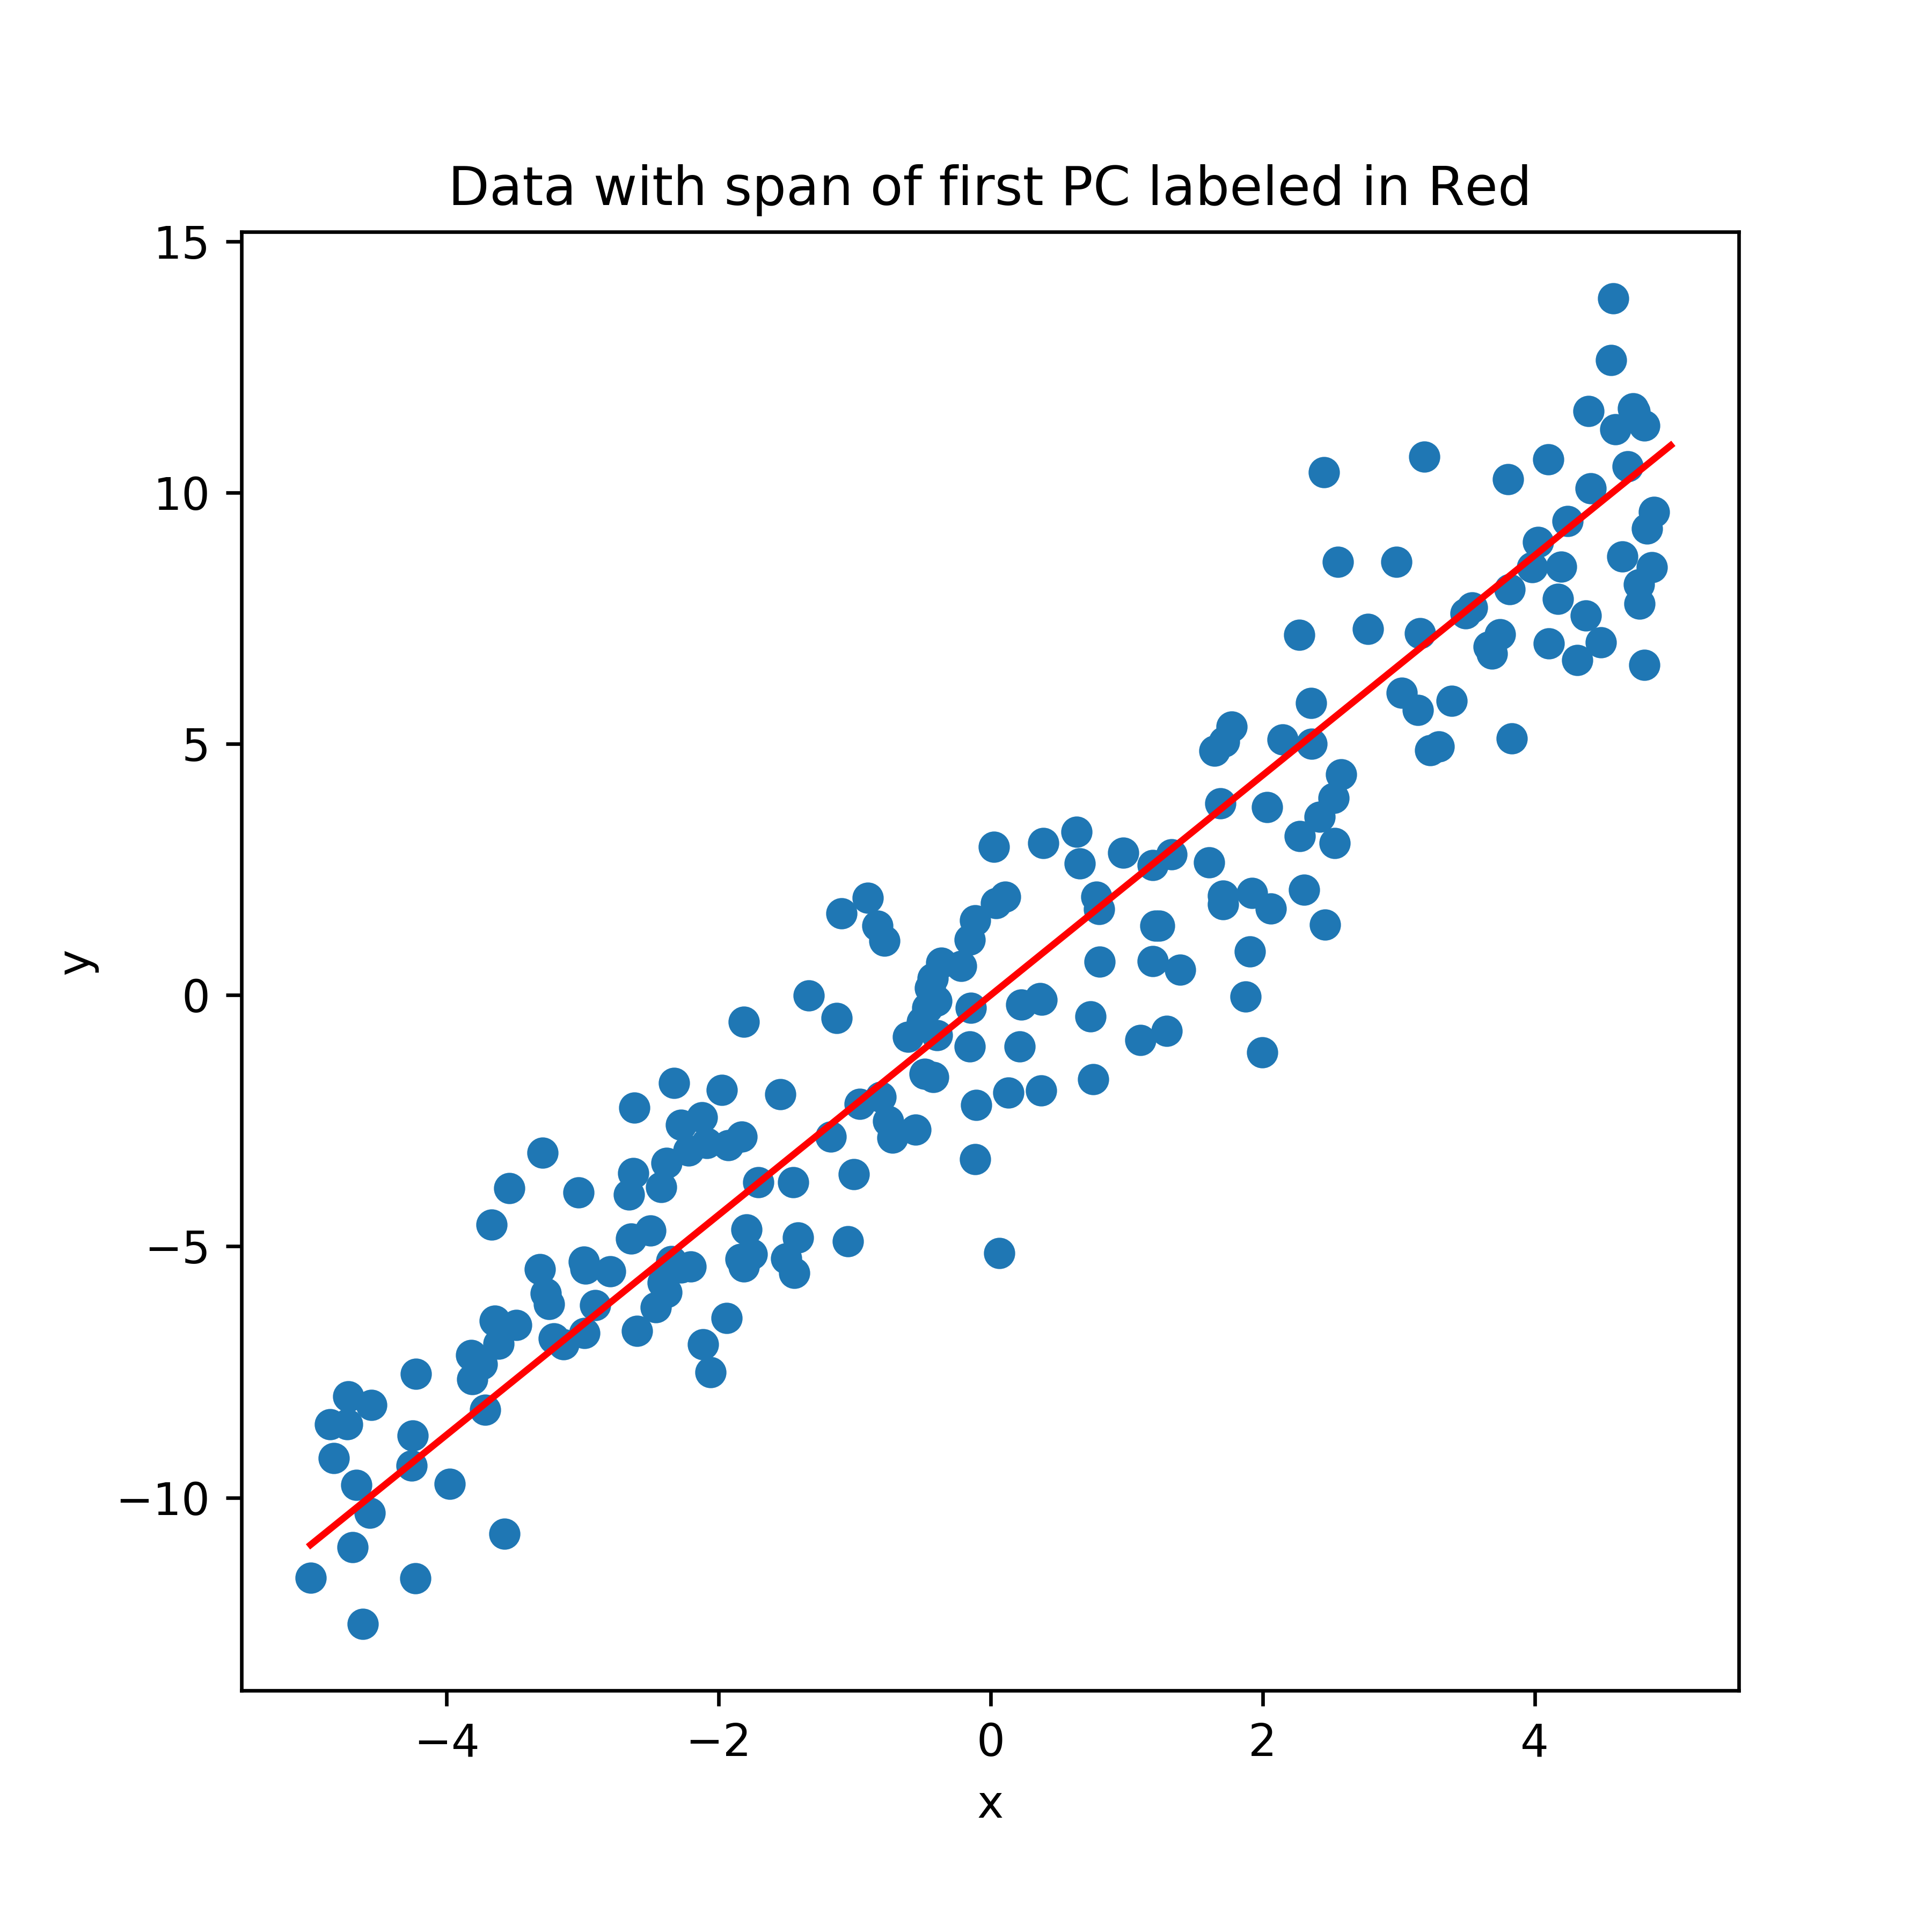
\includegraphics[width=4in]{\bank/svd-pca/figures/2d_data_span.png}
    \end{center}

    Note that this data-set was generated by taking samples of the line $y = 2x$ and adding random noise. 
	}

	\qitem Given the following 3D dataset, draw the direction of the first and second principal components.

  \begin{center}
    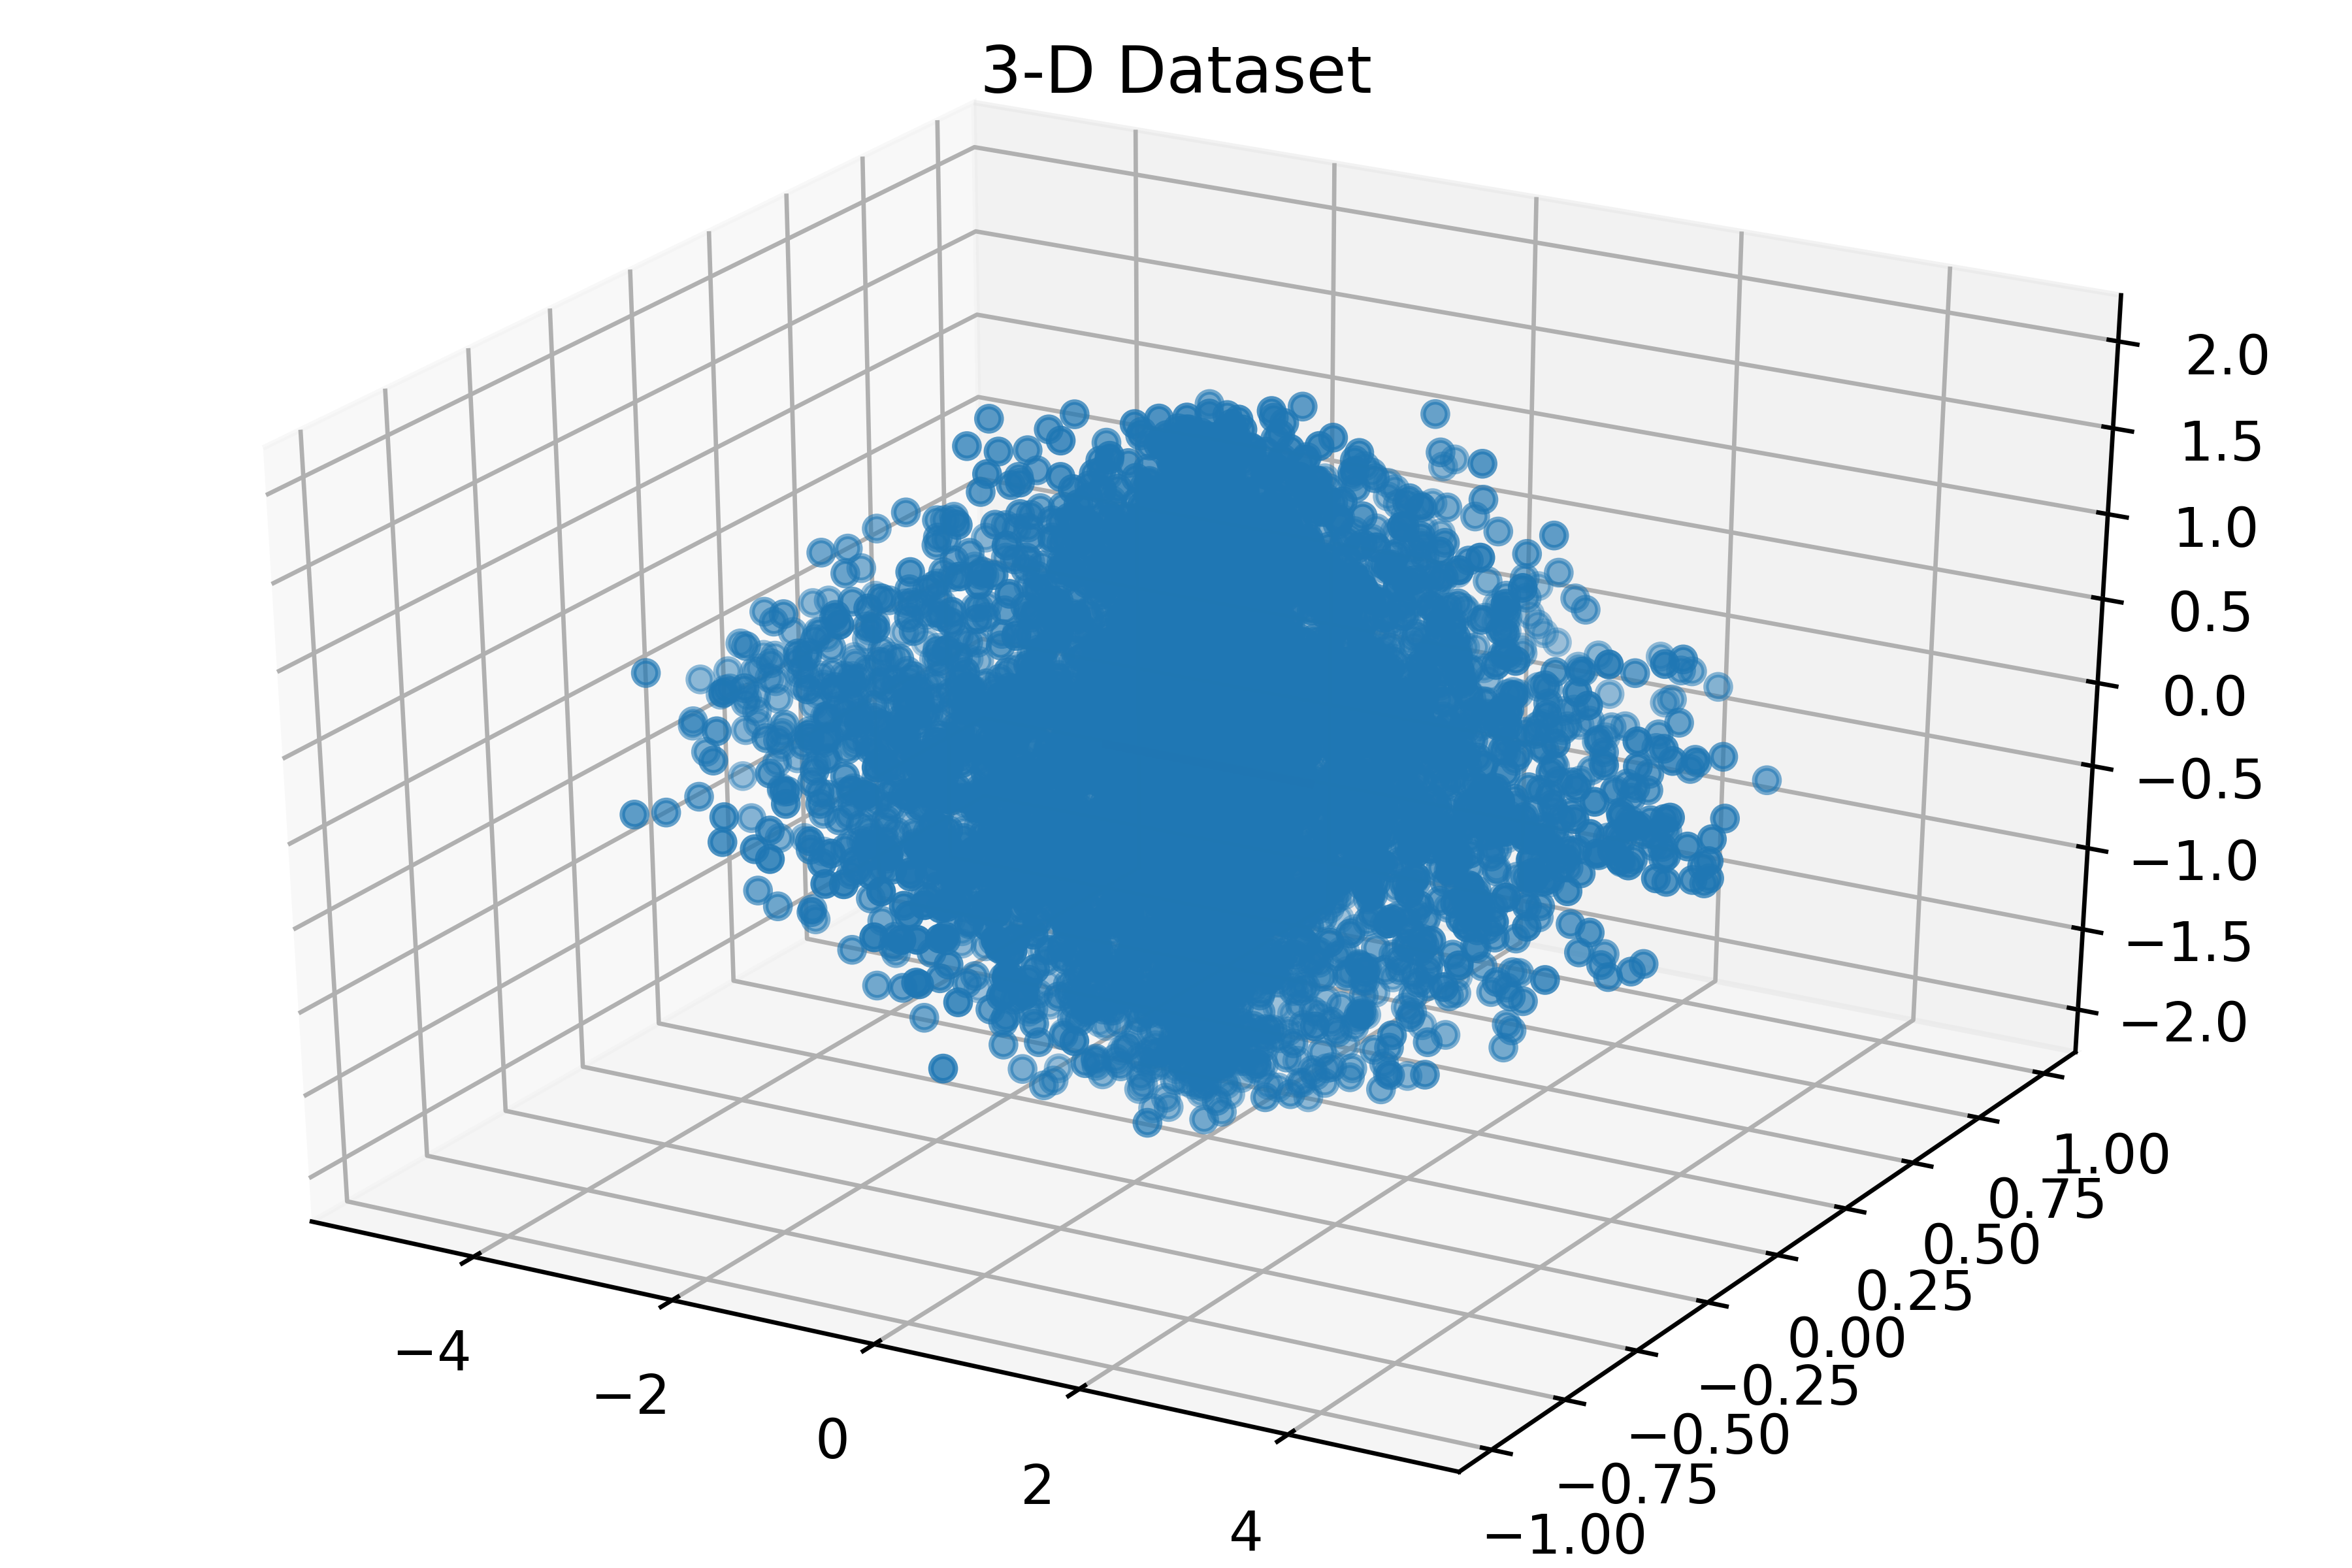
\includegraphics[width=4in]{\bank/svd-pca/figures/3d_data.png}
  \end{center}

	\sol {
    We see that our data is shaped like as a 3D ellipsoid, that is already mean centered at 0. 
    The first principal component will point in the direction of maximal spread, and the second will point in the second most direction of maximal spread, but must be orthogonal to the first.
    Therefore, it will look like the following visually:
    \begin{center}
      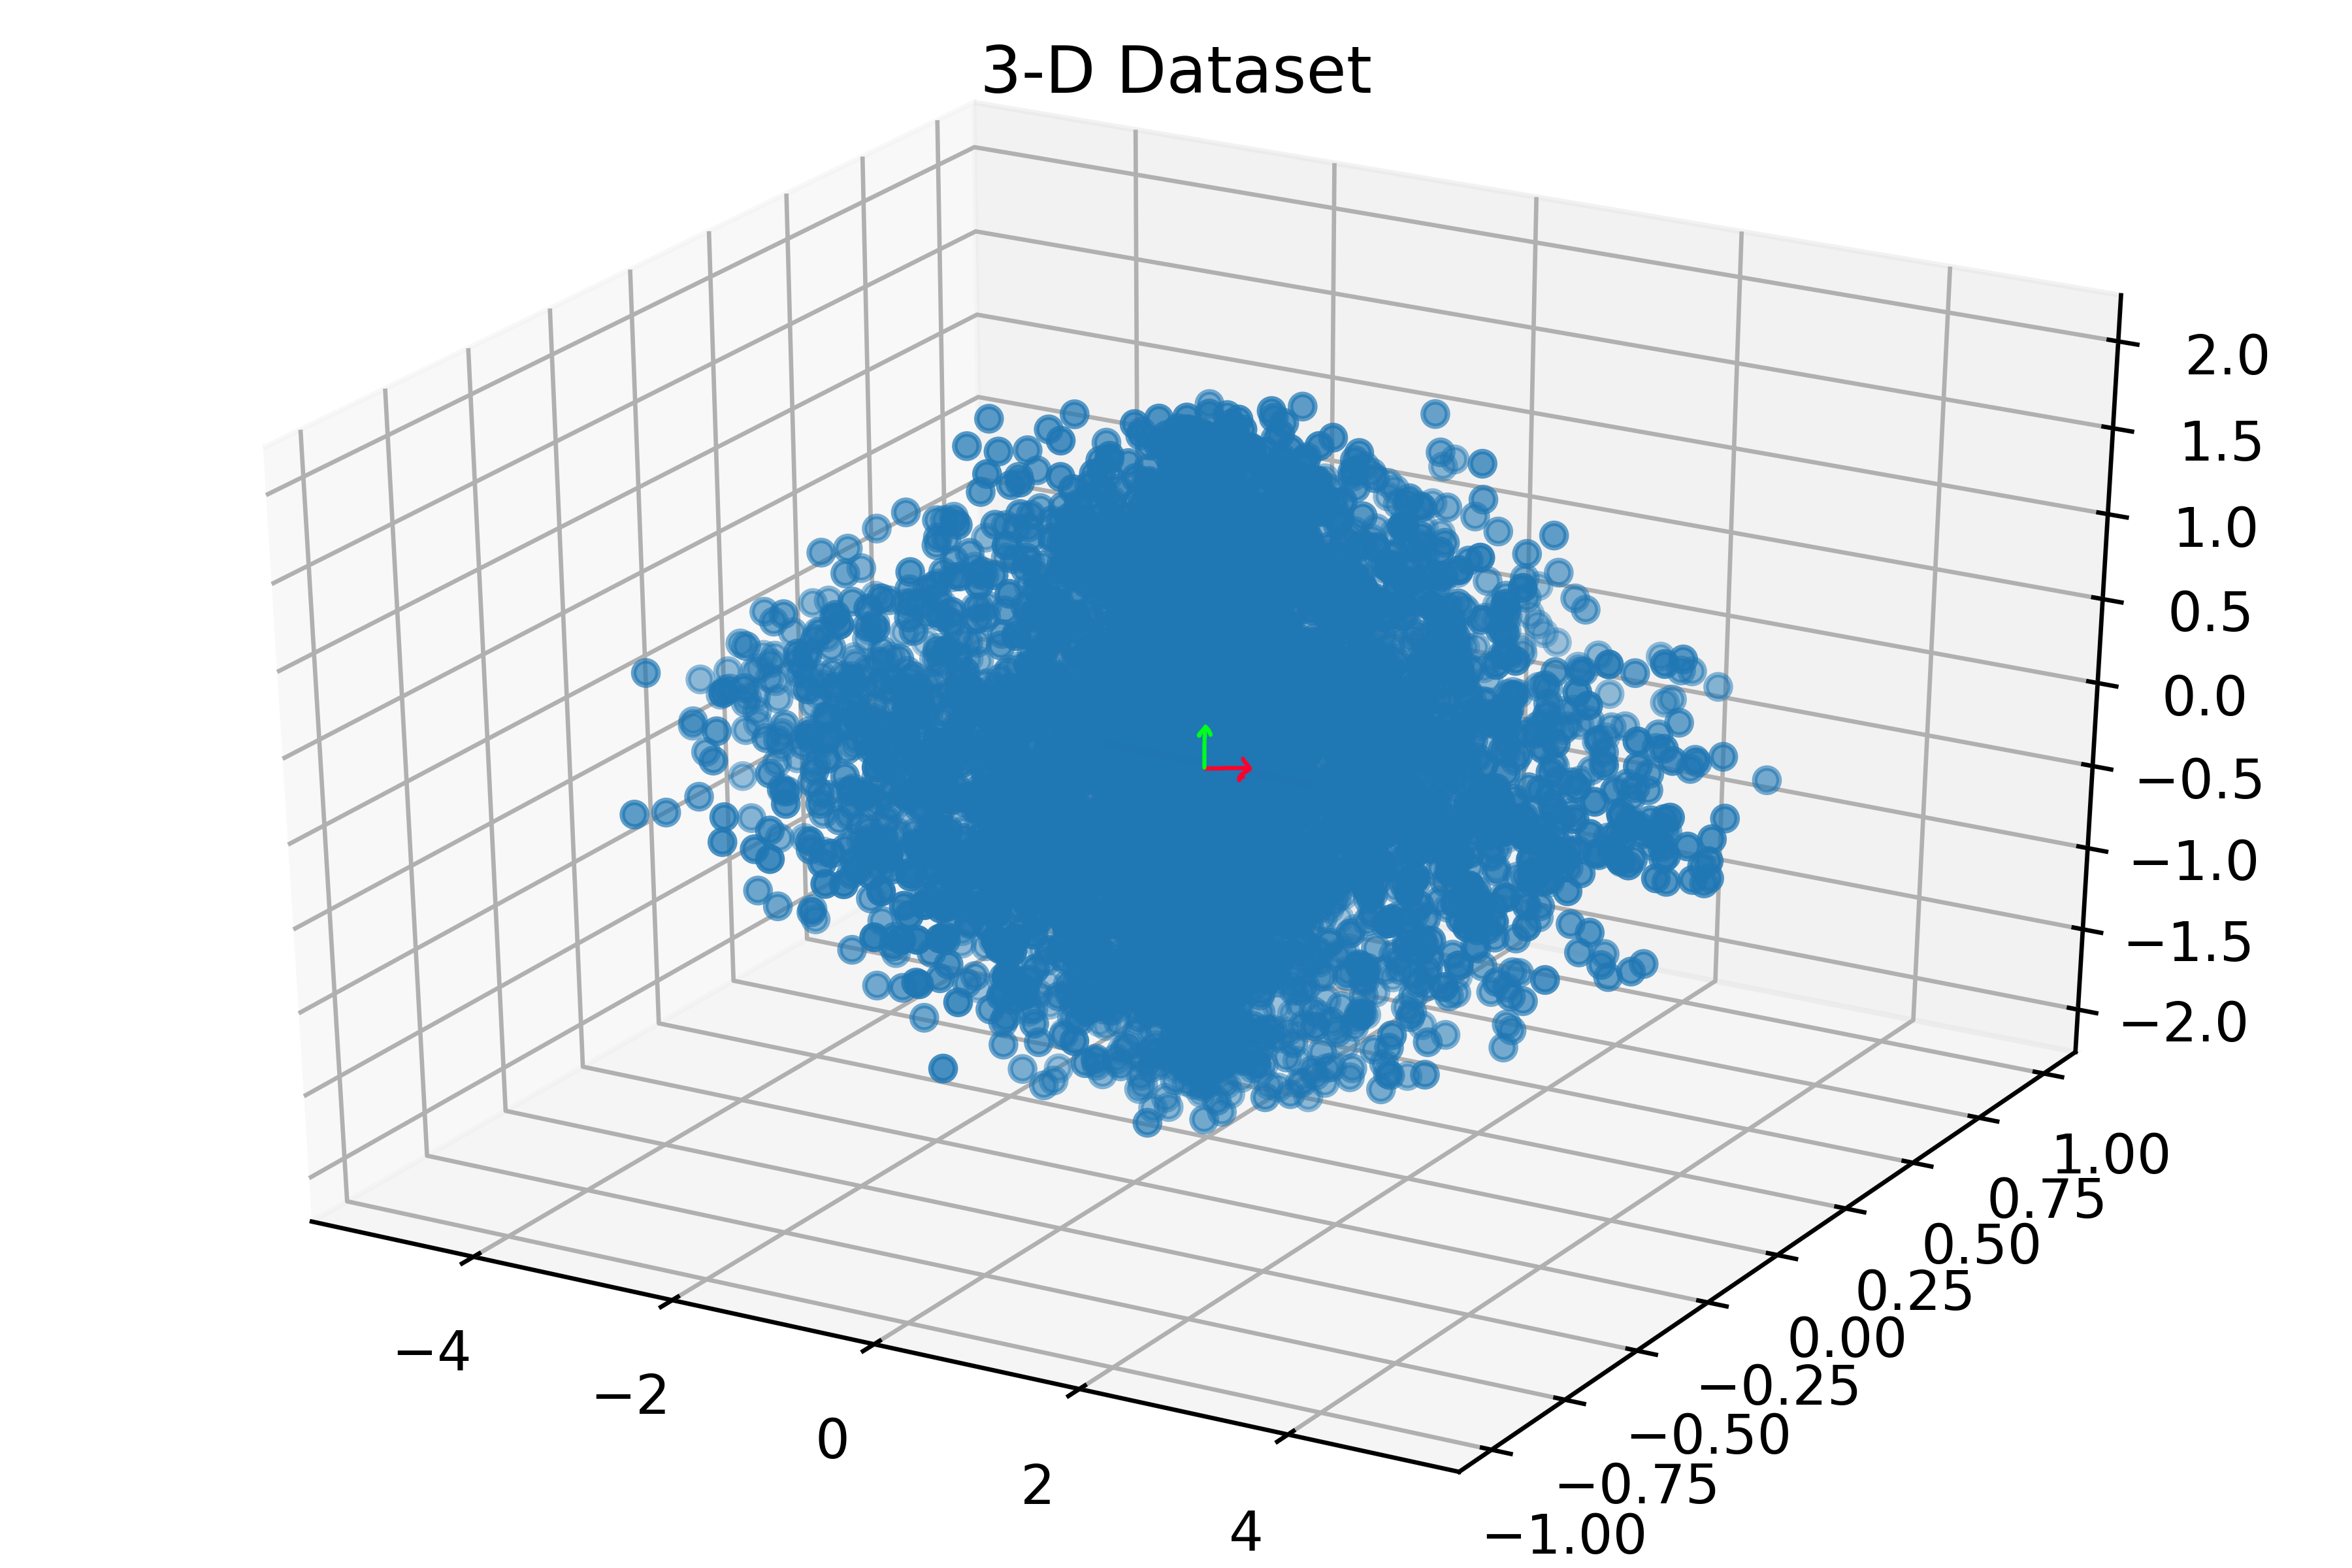
\includegraphics[width=6in]{\bank/svd-pca/figures/3d_data_pc.png}
    \end{center}
    We picked the two most important directions of spread in the data, and we can see what the projection of the data onto the subspace spanned by the first two principal components look like:
    \begin{center}
      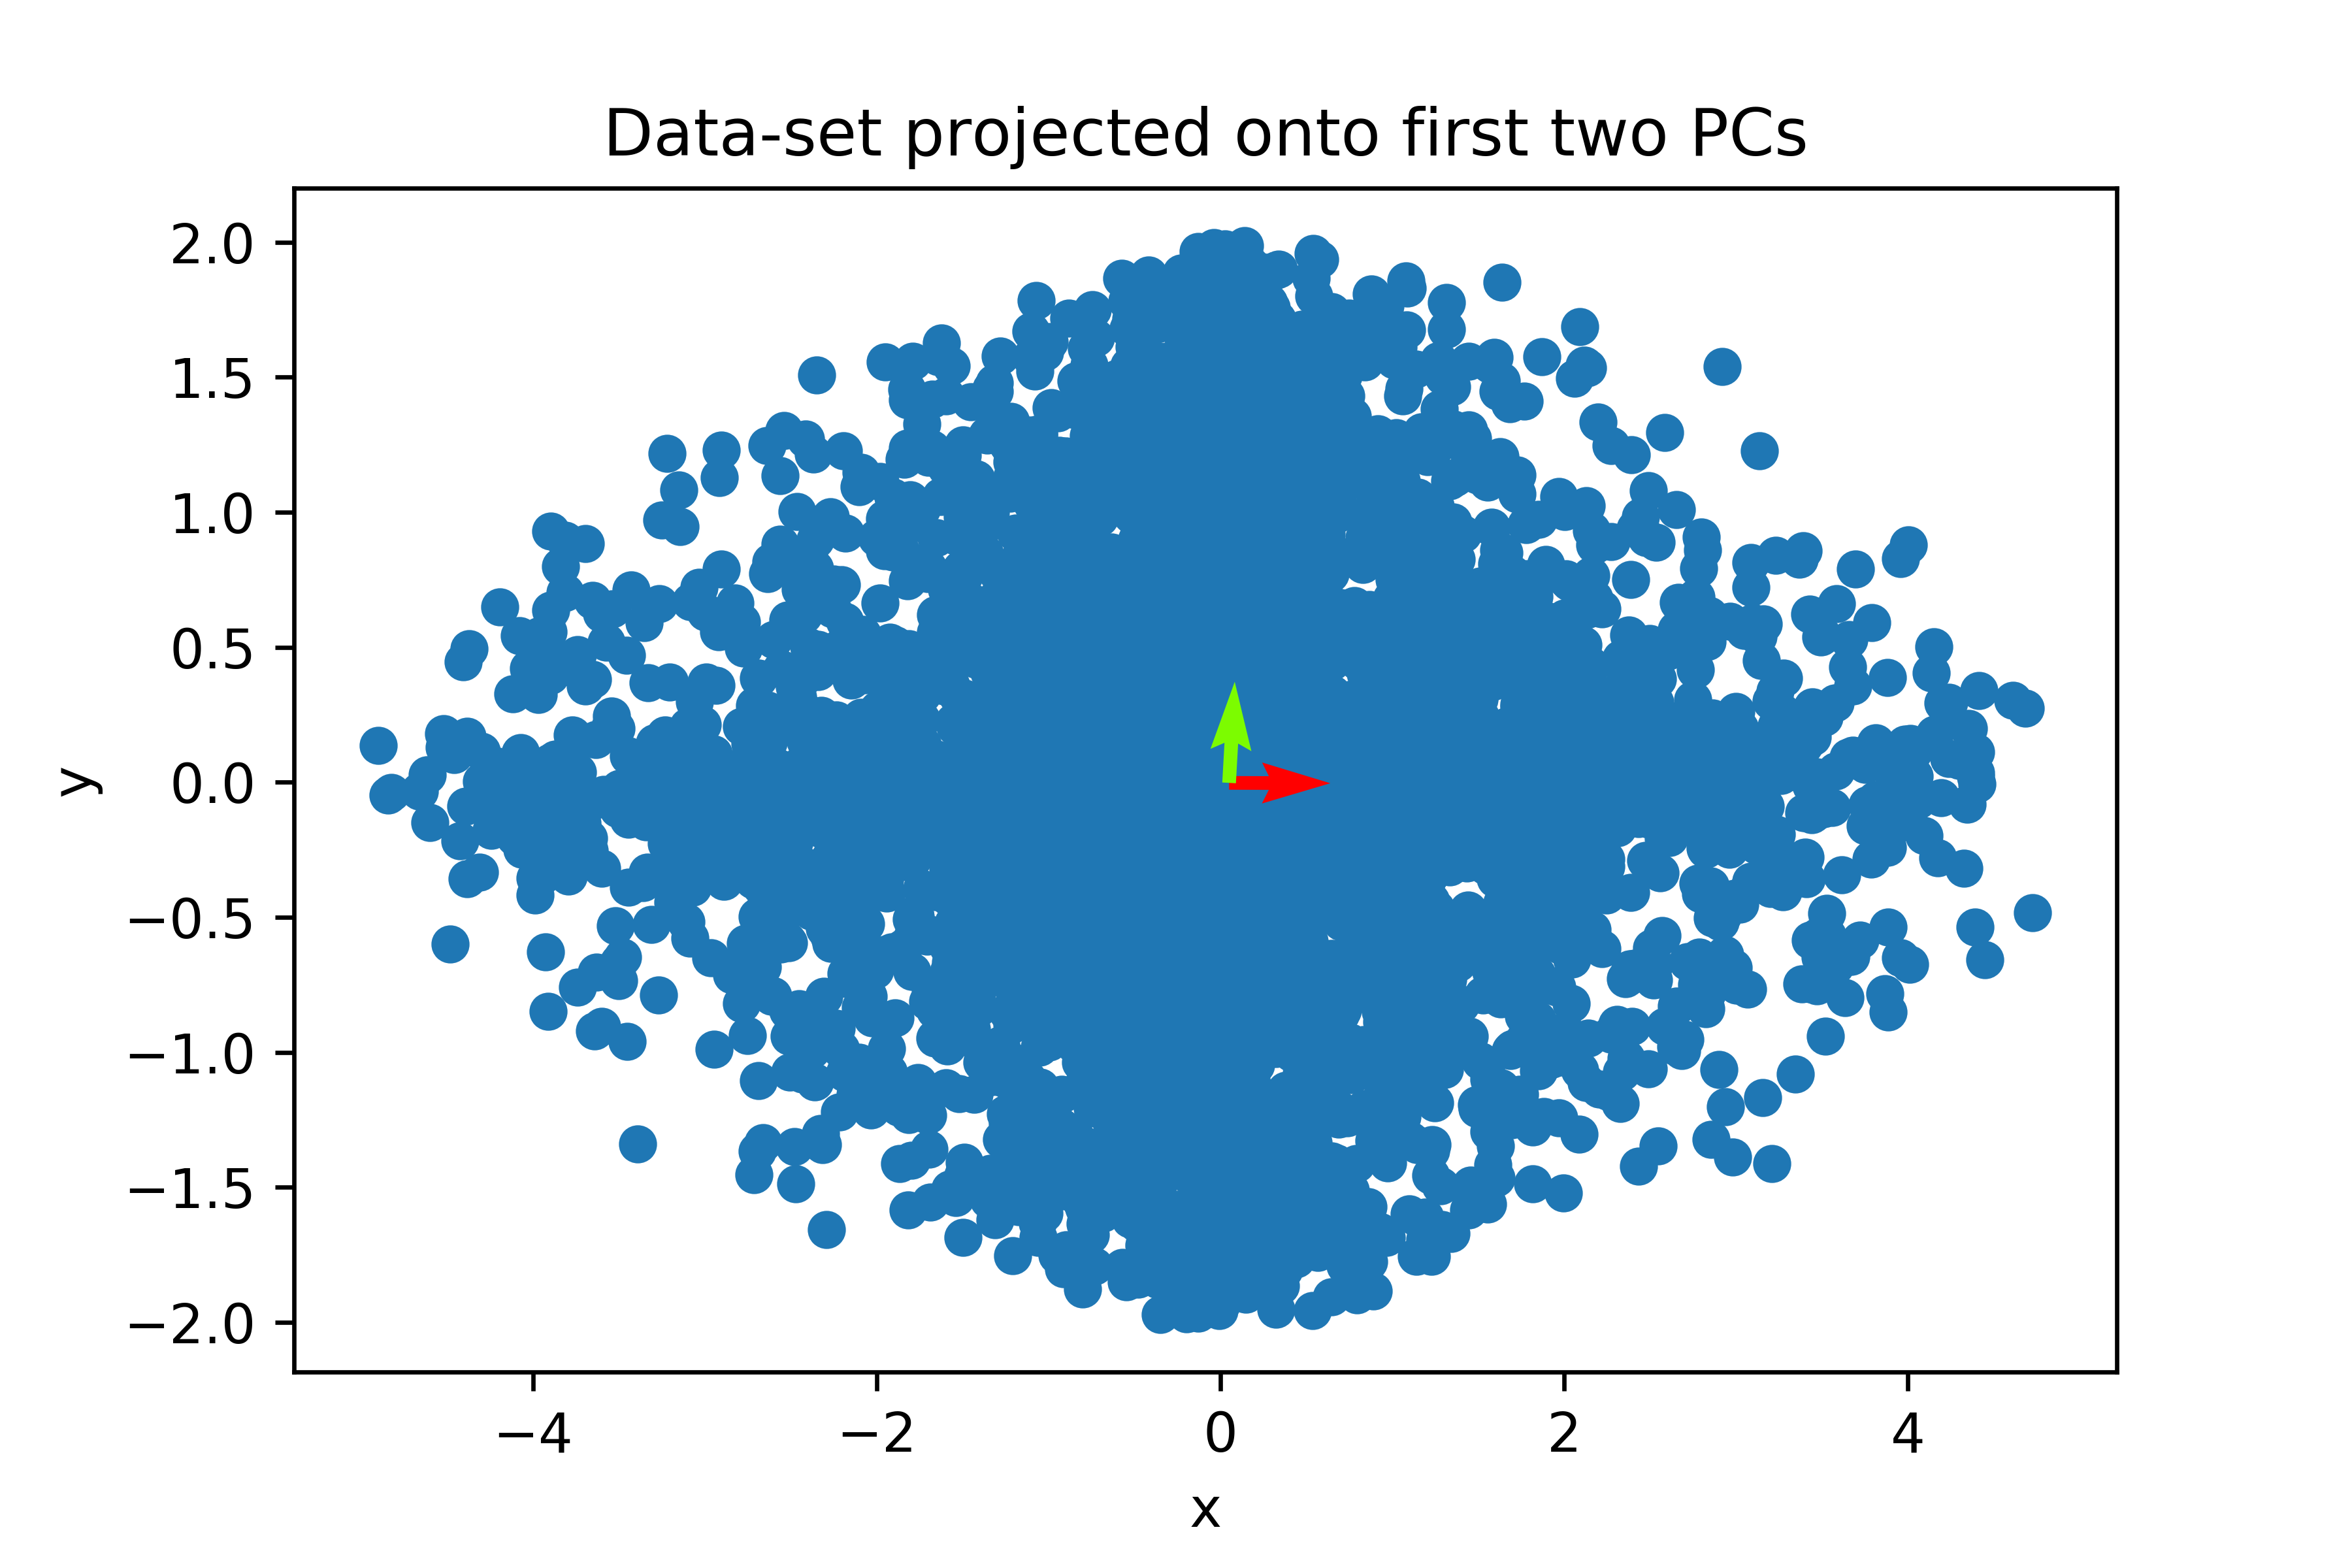
\includegraphics[width=4in]{\bank/svd-pca/figures/3d_data_proj.png}
    \end{center}
    We have taken a three dimensional dataset, and represented it using only two dimensions! 
    You'll see a lot more of this in lab, when we project a much higher dimensional dataset onto a space of 2 or 3 dimensions.
	}

	\qitem Suppose we represent our data matrix $A$ differently. Now, each data point is aggregated as a column vector, instead of a row vector. How does this change how we find our principal components?

	\sol {
    If we aggregated data into a matrix $A$ by columns, instead of rows, then the transpose of this matrix, $A^{T}$ would be how we set up PCA using the row convention.

    Remember that when using the row convention, the principal components came from the $V$ matrix of the SVD. 
    If we wrote $A^{T} = \tilde{U} \tilde{\Sigma} \tilde{V}^{T}$ then the principal components would come from the $\tilde{V}$ matrix. 

    Therefore, we can either transpose our dataset, and perform the SVD, or if we want to keep our data in column form shape, we can realize that $A = (\tilde{U} \tilde{\Sigma} \tilde{V}^{T})^{T} = \tilde{V} \tilde{\Sigma} \tilde{U}^{T} = U \Sigma V^{T}.$
    Therefore, the principal components will \textbf{not} come from the $V$ matrix, but rather, they will come from the $U$ matrix when taking the SVD.
	}

\end{enumerate}